% Full title as you would like it to appear on the page
\chapter{A New Paradigm For Wide-Field Wavefront Sensing}
\label{chap:new_paradigm}
% Short title that appears in the header of pages within the chapter
\chaptermark{A New Paradigm}

\epigraph{What is the most important theme in computer science? [Class responds.] No. It is \textit{abstraction}.}{John Ousterhout in CS 140: Operating Systems, 2020}

\section{Challenges with Previous Approaches}

Keeping telescopes in focus is an art as old as the instruments themselves. Their widespread use spurred the development of theories of optics and aberrations. In 1678, the famed Dutch physicist Christian Huygens proposed that every point that interacts with light may be regarded as the source of a new spherical wave. In 1818, the French physicist Augustin-Jean Fresnel incorporated interference into this model. The resulting Huygens-Fresnel principle is still a widely taught model for wave propagation and provides the physical intution behind reflection, refraction, and diffraction. The paradigm also introduced the notion of the wavefront.

A wavefront is a two dimensional surface over which the phase of the wave is constant. We also overload this diction to refer to aberrations, or two dimensional spatial offsets from a reference wavefront. Figure \ref{fig:wavefront} shows example aberrations to planar and spherical reference wavefronts. 

\begin{figure}[hbt!]
\centering
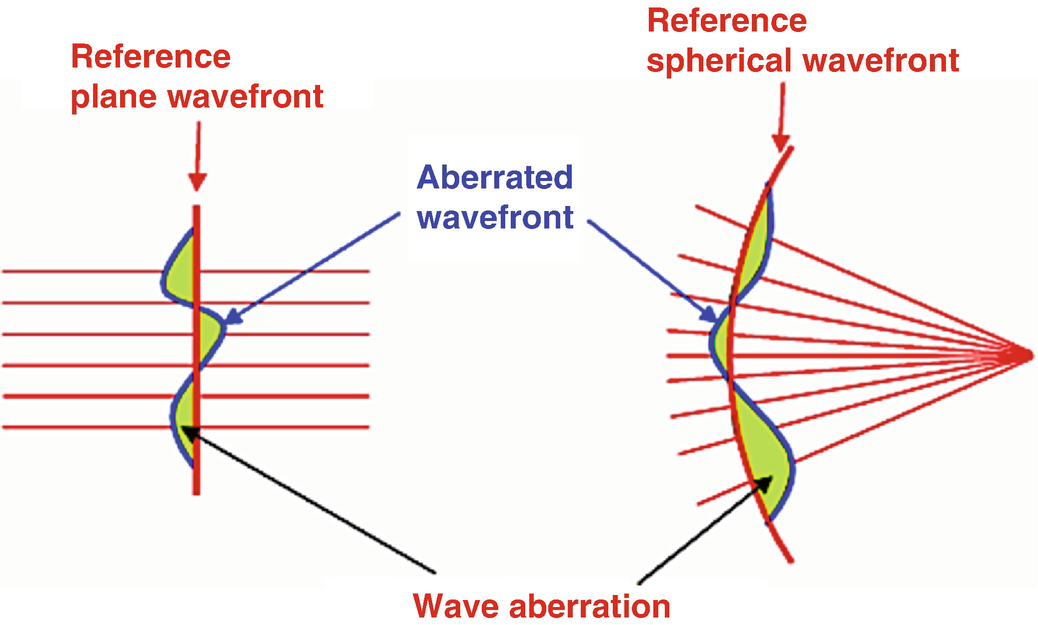
\includegraphics[width=14cm, keepaspectratio]{figs/new_paradigm/wavefront.png}
\caption[Wavefront and Wavefront Aberrations]{Example aberated planar and spherical wavefronts. The horizontal red lines show the direction of propagation. The vertical red line shows the reference wavefront and the blue line shows an example aberrated wavefront. Source: \cite{wavefront_fig}. }
\label{fig:wavefront}
\end{figure}

Wavefronts are useful because the wavefront aberrations in different planes, and through time, largely characterize the image quality of an optic. In the case of ground based telescopes, there are three primary contributions to image quality: the atmosphere, the telescope, and the camera. The field of \textit{adaptive optics} is concerned with controlling deformable mirrors to the optical path to correct for aberrations induced by atmospheric turbulence on 10-100Hz frequencies. However, for wide field telescopes with fields of view on the order of a degree, a common corrections is not possible for the entire field of view. In this context we are primarily concerned with \textit{active optics} which strives to correct the aberrations due to the telescope. New methods of wavefront sensing for active optics is the focus of the first part of this thesis.

One way to characterize the optics of a telescope is through path length differences. For every position in the image plane, we can measure the path differences to points in the entrance pupil. An alternative way to mathematically express this is through an aberrated wavefront defined at the entrance pupil for each position in the image plane. Then the imaging properties can be computed with Fourier Optics. We refer readers who would like to understand this relation further to Goodman's classic Fourier Optics text \cite{goodman2005introduction}. 

There are two thematic approaches to wide field wavefront sensing: zonal and modal. In the zonal approach, the entrance pupil is partitioned into an array of subaperatures. In each of these zones, the wavefront is characterized by its optical path length, local gradient, or local curvature. The wavefront measurement improves with more partitions. The Shack-Hartmann sensor and shearing interferometer are the two most common zonal approaches.

The modal approach treats the wavefront aberration, at a given point in the image plane, as a sum of low order polynomials defined over the entrance pupil. This wavefront measurement improves with higher order polynomial measurements. Modal approaches typically rely on strategically defocused wavefront sensors. The Rubin Observatory focal plane was designed with a modal approach in mind as it does not require lenselets or tweaks to the beam. As described in chapter \ref{chap:aos}, the Rubin focal plane contains four corner wavefront sensors specifically for this purpose.

There are two previously described approaches to wavefront sensing that are relevant for Rubin. The first, by Roodman et. al. \cite{2014roodman}, is the algorithm used for the Dark Energy Camera on the Blanco Telescope \cite{darkenergycamera}. It is based on the Fraunhofer diffraction integral:

\begin{equation}\label{eqn:fraunhofer}
I(x,y) \propto |\mathcal{F}\{P(\rho, \theta \exp(2\pi i W(\rho, \theta) / \lambda))\}|^2
\end{equation}

\noindent where $I$ is intensity; $\mathcal{F}$ is the two-dimensional Fourier transform; $P$ is the pupil function; $W$ is the wavefront; $\lambda$ is the wavelength; and $x,y$ and $\rho, \theta$ parameterize the image and pupil planes respectively. The wavefront is modeled as a sum of orthonormal Zernike polynomials:

\begin{equation}\label{eqn:zernike_decomp}
W(\rho, \theta) = \sum_i a_i Z_i(\rho, \theta)
\end{equation}

\noindent Starting from a set of telescope control parameters, the wavefront coefficients can be computed. Then the Fraunhofer diffraction integral can be used to generate a corresponding intensity image. The difference between the donut images and the images from the forward model,

\begin{equation}\label{eqn:loss}
\mathcal{L} = \sum_{\text{donut d}}||I_{\text{d,true}} - I_{\text{d,forward}}||_2^2
\end{equation}

\noindent can be used as a loss function. Then we can estimate the telescope parameters by using an optimizer to find the parameters that minimize this loss function. This works well when there are a few non-degenerate parameters and the problem remains approximately convex.

While this approach has been successfully applied to the Blanco Telescope, there are two impediments to applying it to the Rubin Observatory. The first is that Rubin has much higher dimensionality and complete degeneracy between some of the parameters of interest. The Blanco Telescope is a prime focus telescope with a single mirror; the Rubin Observatory is a modified Paul-Baker telescope with three mirrors. The Blanco active optics sytem controls 8 parameters; the Rubin active optics system strives to control 50 parameters. The Rubin control parameter optimization surface is highly nonconvex. In addition to these theoretical hurdles, the fast beam of the Rubin optics also necesitates much larger fourier transforms pushing the runtime of the algorithm beyond the 15 seconds we are targeting (see next chapter for more details). 

The second approach is based on the transport of intensity equation (TIE):

\begin{equation}\label{eqn:tie}
\frac{\partial I}{\partial z} = -(\nabla I \cdot \nabla W + I \nabla^2 W)
\end{equation}

\noindent where $z$ is the optical axis. It builds on the curvature wavefront sensing technique developed by Francois, Claude, and Nicolas Roddier \cite{curvaturesensing}. Their key insight was that $\frac{\partial I}{\partial z}$ can be approximated by subtracting two donut images on different sides of focus. Then $W$ in the TIE equation can be solved for in Fourier space or with a Zernike polynomial series expansion. The large central obscuration, fast $f$-number, off-axis distortion and vignetting, and different field positions of intra and extra-focal donuts are four challenges to using curvature sensing for Rubin. Xin et. al. \cite{2015Xin} proposed solutions and extended curvature sensing to estimate the Rubin optics wavefront at four field positions. Below we give a high-level summary of the operations this algorithm performs, on a single wavefront sensor, to estimate the wavefront at the center of the corresponding wavefront sensor:

\begin{enumerate}
\item Crop $N$ pairs of intra-focal and extra-focal donuts \\$\{(D_{\text{intra},1},\ D_{\text{extra},1}), \dots, (D_{\text{intra},N},\ D_{\text{extra},N})\}$.
\item Make initial wavefront estimates $W_0 = 0,\ W_1 = \text{guess}$.
\item Set $i = 1$.
\item While $||W_i - W_{i-1}||_2^2 < \text{tolerance}$ repeat,
\begin{enumerate}
\item Apply nonlinear transformation $f$ which migrates donut image from its field position to the center of the wavefront sensor, based on current wavefront estimate $W_i$. We have $\{(D_{\text{intra},1}^\prime,\ D_{\text{extra},1}^\prime), \dots, (D_{\text{intra},N}^\prime,\ D_{\text{extra},N}^\prime)\}$ where $D_{*,k}^\prime = f(D_{*,k}, W_i)$.
\item Apply correct $g$ for intensity and vignetting differences between the pairs of donuts. We have $\{(D_{\text{intra},1}^{\prime\prime},\ D_{\text{extra},1}^{\prime\prime}), \dots, (D_{\text{intra},N}^{\prime\prime},\ D_{\text{extra},N}^{\prime\prime})\}$ where $D_{*,k}^{\prime\prime} = g(D_{*,k}^\prime, W_i)$.
\item Set $(\partial_z I)_k \propto D_{\text{intra},k}^{\prime\prime} - D_{\text{extra},k}^{\prime\prime}$.
\item Solve TIE for $W_{i+1}$ with $(\partial_z I)_k$ by series expansion.
\item Set $i = i + 1$.
\end{enumerate}
\item Return $W_i$ as wavefront for the center of the wavefront sensor.
\end{enumerate}

\noindent Afer this process the algorithm uses the wavefront estimates at the center of the four corner wavefront sensors to constrain 50 telescope control parameters (these parameters are described in the next chapter). 

This approach has been developed by a dedicated team over the last decade. Parts of the algorithm, such as step 4 (d) are mature and have been validated on real data \cite{cwfs_comparison}. However, despite significant effort, the code for the full algorithm on Rubin remains incomplete. Thus it is difficult to benchmark or compare to alternatives.

The primary challenge on theoretical grounds is the convergence. There are no convergence gaurentees. The wavefront estimate may not improve between the iterations in step 4. Some tests suggest that the algorithm typically converges for small perturbations to the nominal optics configuration. However, for large perturbation the transformations $f$ and $g$ will have more error. A different strategy might be required.

The algorithm is also fairly computationally expensive. It takes approximately 15 seconds to perform 10 iterations of step 4 on 10 pairs of donuts. However, a typical wavefront sensor image contains close to a thousand donut images. A lot of potentially useful donut information is ignored.

There are also a few challenges on practical grounds. The functions $f$ and $g$ used in step 4 depend on the wavefront estimate and are fairly complicated. This makes the algorithm challenging to interpret and debug. Also, since $f$ and $g$ depend on the wavefront estimate, it is difficult to characterize the error in the full algorithm, because each step depends on the preceeding steps. 

After spending a year supporting efforts to implement this algorithm, I realized the prudence in developing an alternative approach. I sought to develop an algorithm that was simple, transparent, robust, low-latency, and high-throughput. The next two sections develop two key paradigms behind the algorithm.

\section{The Double Zernike Polynomials}

The Zernike polynomials are a sequence of polynomials $\{Z_i\}$ that are widely used to characterize wavefronts in optics \cite{zernike}. They are defined over a unit disk, or annulus, and normalized such that

\begin{equation}\label{eqn:zernike_norm}
\int_{R_{\text{inner}}}^{R_{\text{outer}}} \int_0^{2\pi} Z_i(\rho,\theta)Z_j(\rho,\theta)d\rho d\theta = \delta_{ij}
\end{equation}

\noindent Figure \ref{fig:zernike} shows the first 21 Zernike polynomials. For characterizing a wavefront in the pupil plane we follow the convention of using $Z_4-Z_{21}$ by Xin et. al. \cite{2015Xin}. The first three polynomials are ignored because while they effect the position of the image, they do not impact the image quality. The polynomials beyond 21 are ignored because they are only weakly excited by typical Rubin perturbations.

\begin{figure}[hbt!]
\centering
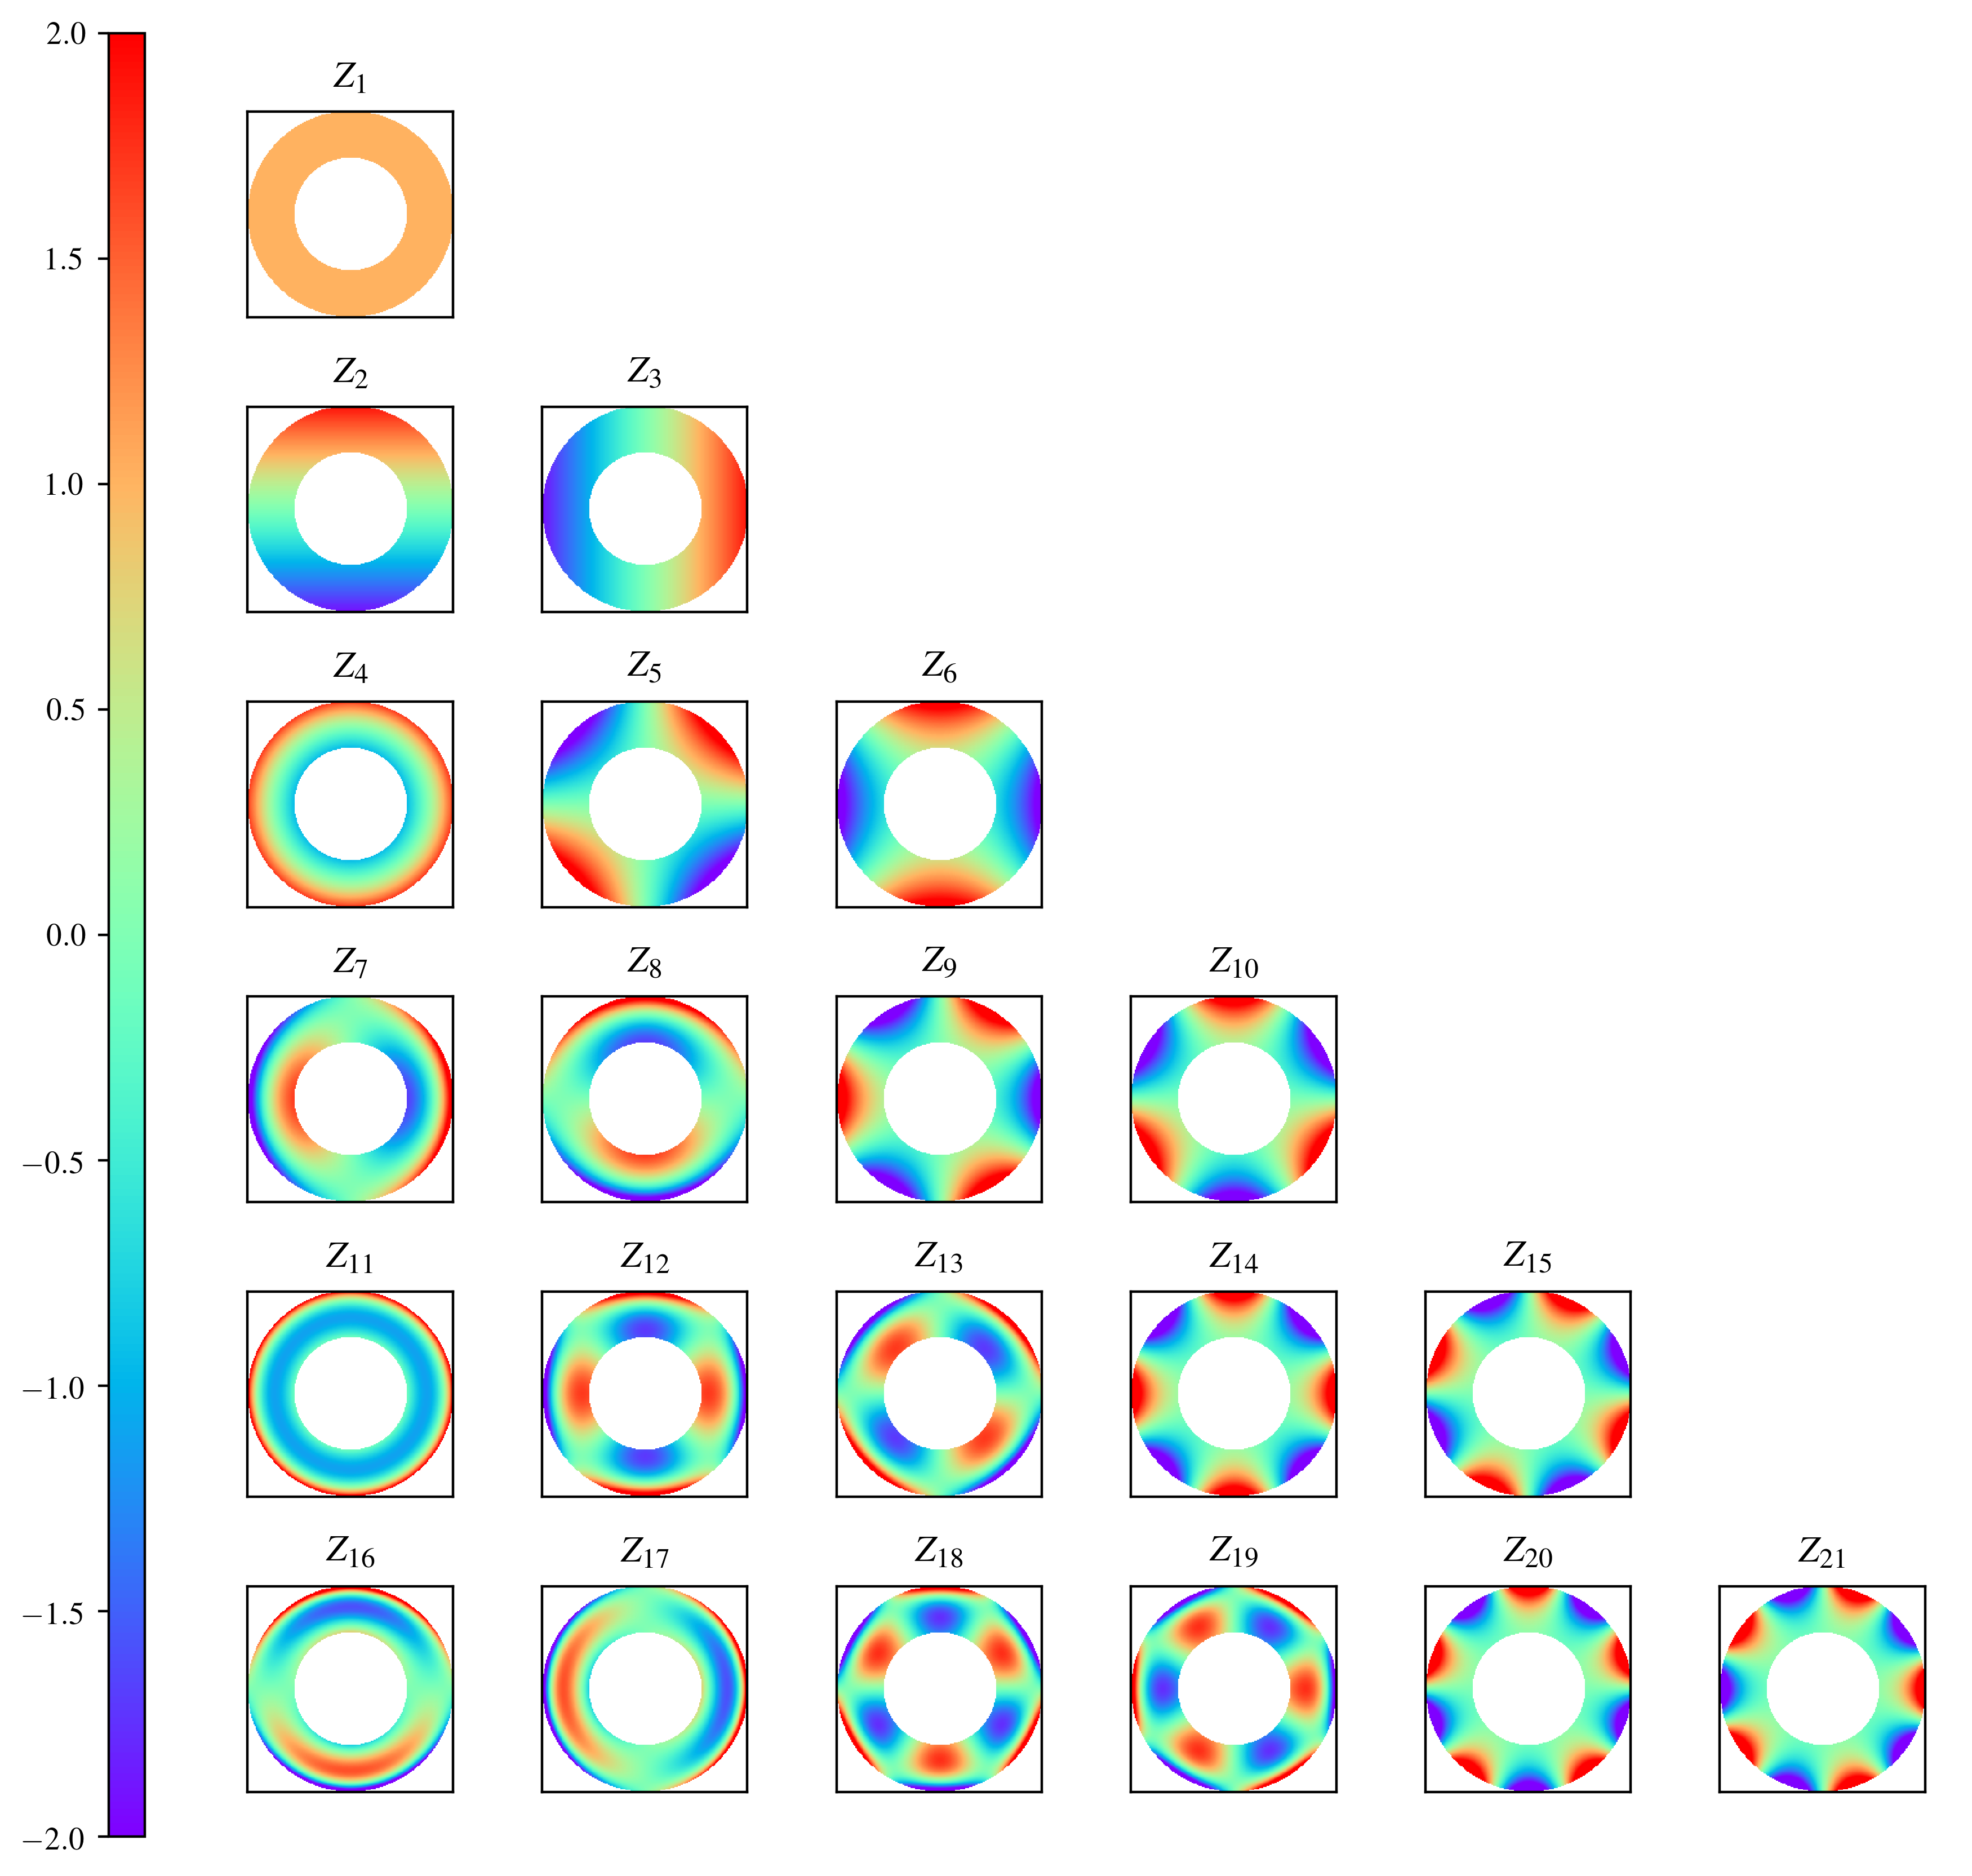
\includegraphics[width=14cm, keepaspectratio]{figs/new_paradigm/zernikes.png}
\caption[Zernike polynomials]{The Zernike polynomials $Z_1$ throught $Z_24$ with the Noll index scheme. The obscuration of the annular domain is consistent with the obscuration in the Rubin optics.}
\label{fig:zernike}
\end{figure}

For small telescopes, this basis can be used to characterize the wavefront in the entrance pupil. For wide-field telescopes like the Rubin Observatory, the wavefront changes non-trivially across the field of view. Thus the wavefront is a four dimensional function of both the entrance pupil and focal plane. One way to model this would be to have another polynomial basis $\{P_i\}$ for the focal plane $x,y$. Then we could write the full wavefront as $W(x,y,\rho, \theta) = \sum_i \sum_j \beta_{ij} P_i(x,y) Z_j(\rho, \theta)$. The coefficients $\beta$ are indexed by the image plane index $i$ and pupil plane index $j$. The double Zernike polynomials are the $P_i(x,y) Z_j(\rho, \theta)$ where the field polynomials are circular Zernike polynomials $P_i = Z_i$ \cite{doublezernike}. Thus $\beta_{ij}$ is the mode of circular polynomial $Z_i$ in the focal plane, and annular polynomial $Z_j$ in the image plane.

In practice we also truncate the focal plane index. This leaves us with a finite set of coefficients to represent the full wavefront across the pupil and focal planes. We found that for the Rubin Observatory, most of the aberration power is concentrated in the first three focal plane polynomials. We simulated 500 perturbed telescope states and numerically calculated the double Zernike coefficients out to index 36. Then we studied the fraction of the aberrated wavefront contained in the first $k$ focal plane Zernikes. We found that the first three polynomials capture 90\% of the wavefront. These first three polynomials are a constant offset, a tip-plane, and a tilt-plane - collectively they define a plane. We suspect a similar pattern holds for other wide field telescopes. It suggests that the 54 double Zernike coefficients $\beta_{ij}$where $1 \leq i \leq 3$ and $4 \leq j \leq 24$ offer a good characterization of the wavefront.

\begin{figure}[hbt!]
\centering
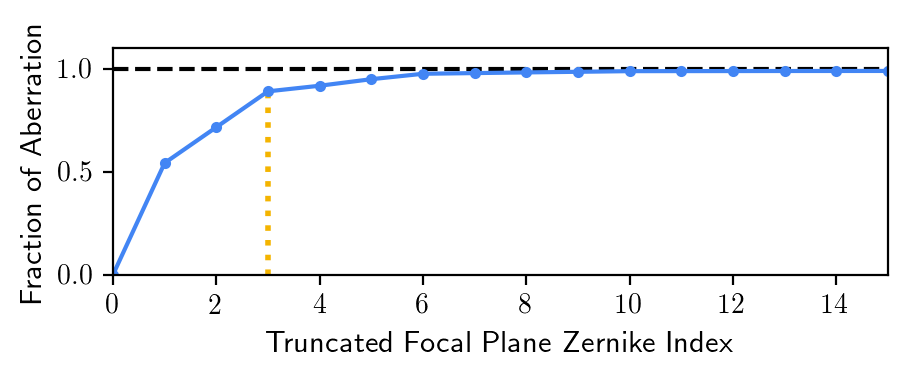
\includegraphics[width=14cm, keepaspectratio]{figs/new_paradigm/truncated.png}
\caption[Aberration Power in Focal Plane Zernikes]{The fraction of the aberration that is present in the first $k$ focal plane Zernike polynomials, where $k$ is the truncation index on the x-axis.}
\label{fig:truncated}
\end{figure}

This separation of the wavefront into pupil and focal plane components is key to this work. Our key insight was as follows. At any point in the image plane, we can use the image to constrain the pupil wavefront at that position - we deem this the \textit{local} wavefront. Then we can interpolate the focal, or \textit{global}, wavefront from all the local estimates. In section \ref{sec:decomposing}, we describe techniques that are very well suited for each of these subproblems. Before then, we summarize recent progress in neural network based phase estimation.

\section{Neural Network Based Phase Estimation}
The potential for neural networks to learn the non-linear mapping between intensity patterns and aberrations in the pupil plane was first recognized in 1990 \cite{1990NatureMLAO}. Shortly afterwards, this potential was realized as neural networks were deployed to detect turbulence induced distortion on the Multiple Mirror Telescope \cite{1991NatureMLAO} and to detect aberrations in the primary mirror of the Hubble Space Telescope \cite{1993HubbleMLAO}. Others expanded this concept to predict more wavefront components \cite{1992SPIE.1706..113J}, incorporate temporal history \cite{1996ESOC...54...95L,1997ApOpt..36..675M}, compare reconstruction methods \cite{2006OExpr..14.6456G}, and better characterize atmospheric turbulence \cite{2008ISTSP...2..624W}. 

In the past decade, convolutional neural networks (CNNs) \cite{726791} have re-emerged and spurred dramatic advances in computer vision \cite{10.5555/2999134.2999257, 10.5555/2999792.2999897, 10.1007/s11263-015-0816-y,7780459}. This has created new possibilities for wavefront sensing in astronomy. In \cite{2018OptL...43.1235P}, the authors created a CNN that could estimate the wavefront from a single PSF image. They used these estimates as initial starting points in a gradient-based optimization and showed this was superior to using random samples. \cite{2019OExpr..27..240N} showed wavefront sensing performance could be improved by introducing a preconditioner to broaden the PSF and create more intensity structure for the neural network to exploit. This brings up interesting new design possibilities for wavefront sensors. While conventional Lyot-based low order wavefront sensing methods have a limited dynamic range due to their linear recovery, \cite{2020OExpr..2826267A} showed that a CNN can extend the aberration range over which the wavefront can be estimated by an order of magnitude.

Previous work on machine learning based wavefront sensing focuses on sensing the full wavefront aberration. Here we focus on sensing the optics wavefront, across the field of view, in the midst of the dominant atmospheric contribution. This problem presents new challenges, such as how to best aggregate intensity information from throughout the field of view to suppress the spatially correlated error due to the turbulence contribution. Our approach is comprised of only two steps, is easy to characterize, and can process each donut image in 6 \textit{milliseconds}.

\section{Wavefront Estimation Framework}
\label{sec:decomposing}

The optics wavefront $W_{\text{opt}}$ is a function of two separate planes: the pupil plane parameterized by $(u,v)$ and the focal plane parameterized by $(x,y)$. We use the double Zernike polynomial basis \cite{doublezernike} to represent the optics wavefront, 
\begin{equation}W_{\text{opt}}(u,v,x,y) = \sum_{i=1}^k\sum_{j=1}^m\beta_{ij}Z_i(u,v)Z_j(x,y)\end{equation}
\noindent where $\beta_{ij}$ are the coefficients, $Z_i$ are annular Zernike polynomials over the pupil, and $Z_j$ are circular Zernike polynomials over the focal plane. The goal of wavefront sensing is to estimate these coefficients $\beta_{ij}$ from the $n$ donut images $D_i$ positioned across the wavefront sensors (see Figure \ref{fig:focalplane}). Let the position of donut $i$ be $x_i,y_i$ and the defocus offset of the corresponding sensor be $z_i$. The wavefront sensing problem is to find $f$ such that
\begin{equation}\beta = f((D_1,x_1, y_1, z_1), \dots, (D_n, x_n, y_n, z_n))\end{equation}

We break this into two subproblems.

\begin{enumerate}
	\item Estimate the local wavefront with a CNN at each donut position.
	\item Interpolate the global wavefront from the local wavefront estimates across the focal plane.
\end{enumerate}

\noindent These steps are outlined in Figure \ref{fig:twostep}. 

\begin{figure}[hbt!]
\centering
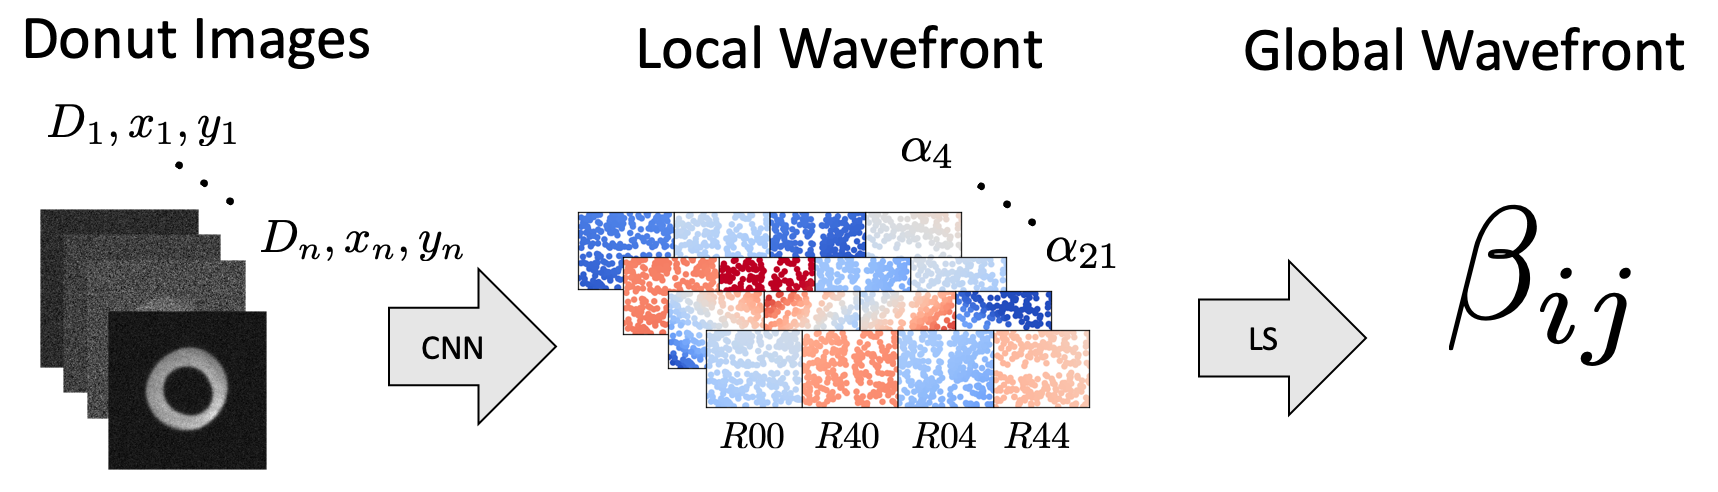
\includegraphics[width=14cm, keepaspectratio]{figs/new_paradigm/twostep.png}
\caption[Two Step Approach To Wavefront Sensing]{In the first step, a convolutional neural network (CNN) processes each donut crop on the four wavefront sensors. In the second step, from each local wavefront coefficient we interpolate three global wavefront coefficients with least squares optimization (LS).}
\label{fig:twostep}
\end{figure}

\subsection{Estimating Local Wavefronts}
In the first subproblem, we estimate the total local wavefront $w_{\text{tot}}(u,v)$ from donut $D_i$ at position $x_i, y_i, z_i$. The intensity in the donut image is related to the total local wavefront by the Fraunhofer diffraction integral (equation \ref{eqn:fraunhofer}). We represent the local wavefront in a basis of annular Zernike polynomials over the pupil, such that the total local wavefront for donut $i$ at position $x_i, y_i$ is
\begin{equation}
w_{\text{tot}}(u,v) = \sum_j \alpha_{ij}Z_j(u,v)
\end{equation}
Convolutional neural networks (CNNs) are particularly well suited for processing images and learning nonlinear mappings. We develop a CNN $\varphi$ to solve the inverse problem of estimating $\alpha_{ij}$ for $j = 1\ \dots m$ from $(D_i,x_i,y_i,z_i)$ . In chapter \ref{chap:cnn} we describe the implementation of this model in detail. 

\subsection{Interpolating the Optics Wavefront}

In the second subproblem, we aggregate the local estimates from the first subproblem to constrain $\beta$. The total local wavefront at position $x_i,y_i$ is related to the optics wavefront via
\begin{equation}w_{\text{tot}}(u,v) = W_{\text{opt}}(u,v|x_i,y_i) + \epsilon(u,v|x_i,y_i)\end{equation}
where $\epsilon$ represents the atmospheric turbulence contribution to the wavefront. Let $\mathcal{Z}$ be defined such that $\mathcal{Z}_{ij} = Z_j(x_i,y_i)$. Then for $i = 1,\dots,m$ we have
\begin{equation}
\alpha e_i = \mathcal{Z} \beta e_i + \epsilon
\end{equation}
where $e_i$ is the $i$th unit vector. Then combining the $\alpha$ from the previous subproblem, and computing the corresponding $\mathcal{Z}$, allows us to solve for $\beta$,
\begin{equation}
\beta = \text{argmin}_{\beta}\left \{\sum_{i=1}^m \ell(\alpha e_i, \mathcal{Z} \beta e_i)\right\}
\end{equation}
where $\ell$ is a convex loss function. Algorithm \ref{alg:main} shows the psuedocode. 

\begin{algorithm}
    % \SetKwInOut{Input}{Input}
    % \SetKwInOut{Output}{Output}
    % \underline{function Estimate Optics Wavefront}\\
    % \Input{combined wavefront sensor image $I \in \mathbb{R}^{N\times N}$}
    % \Output{optics wavefront $\beta \in \mathbb{R}^{k \times m}$}
    \text{given image} $I \in \mathbb{R}^{N \times N}$\\
    \text{initialize local wavefront estimate} $\alpha \in \mathbb{R}^{n \times m}$\\
    \text{initialize global Zernike basis} $\mathcal{Z} \in \mathbb{R}^{n \times k}$\\
    \For{\text{donut} $i$ \text{ in } 1\dots n}
    {
        $D_i = \text{Crop}(I, x_i, y_i)$\\
        $\alpha[i,:] = \varphi(D_i, x_i, y_i, z_i)$\\
        \For{\text{zernike} $j$ \text{ in } 1\dots k}
        {
        	$\mathcal{Z}[i,j] = Z_j(x_i, y_i)$
        }
    }
    \text{initialize optics wavefront} $\beta \in \mathbb{R}^{k \times m}$\\
    \For{\text{local Zernike } $i$ \text{ in } $1 \dots m$}
    {
      $\beta[:,i] = \text{argmin}_{\beta[:,i]}\ \{\ell(\alpha[:,i], \mathcal{Z}\beta[:,i])\}$\\
    }
    \text{return } $\beta$\\
    \caption{estimates the optics wavefront from donut images.}
    \label{alg:main}
\end{algorithm}

The dominant source of error is the atmospheric turbulence contribution to the wavefront. This error is correlated on scales of arcminutes. By processing donuts with reasonable separation and between different wavefront sensors we are able to suppress this error by roughly a factor of $1 / \sqrt{n}$ where $n$ is the number of donuts used.

There are two parameters of our algorithm that must be set based on the telescope: the number of Zernike coefficients to use for the pupil $m$, and the number of Zernike coefficients to use for the focal plane $k$. For the Rubin Observatory we use Zernikes $Z_4$ through $Z_{21}$ for the pupil plane. The first three coefficients do not impact image quality, so we exclude them. We truncate the basis at $Z_{21}$, a convention set by \cite{2015Xin}, as the higher order terms have very small coefficients in practice. We use $Z_1$ through $Z_3$ for the focal plane. Our simulations show that 90\% of the optics wavefront is contained in this truncated basis.

There are two benefits to dividing the wavefront estimation problem into these two subproblems that are worth highlighting. The first is the useful intermediate data products. The local wavefront coefficients $\alpha$, which are estimated in the first subproblem, are physically meaningful. Telescope operators can track them during operations and gain further insight into the system. This adds an additional layer of transparency and robustness.

The second benefit is that it makes deep learning approaches feasible. Deep neural networks must be trained on large datasets to avoid overfitting. The input to the original problem is four wavefront sensor images, or up to thousands of donut images. The raytracing necessary to simulate even a single input sample is computationally expensive. In our first subproblem however, the input is only a single donut image. This reduces the computation required to produce a training sample by three orders of magnitude and makes it possible to generate simulated datasets that are sufficient for training deep neural networks. In chapter \ref{chap:cnn}, we highlight the power of these models.

